\section{History of Speech Synthesis}
\label{history_speech_synthesis}
Speech synthesis can be defined as the artificial generation of speech. Nowadays the process has been facilitated due to the improvements made during the last 70 years in computer technology, making the computer-based speech synthesis systems lead the way supported by their flexibility and their easier access compared to mechanical systems. However, after the first resonators built by Kratzenstein, the fist speaking machine was built and presented to the world in 1791, and was obviously mechanic.

\subsection{Acoustical-Mechanical Speech Machines}
The speech machine developed by von Kempelen incorporated models of the lips and the tong, enabling it to produce some consonants as well as vowels. Although Kratzenstein presented his resonators before von Kempelen his speech machine, von Kempelen started his work quite before, publishing a book where he described the studies made on human speech production and the experiments he made with his speech machine over 20 years of work \cite{vonKempelen}.  

The machine was composed by a pressure chamber, acting as lungs, a vibrating reeds in charge of the functions of the vocal cords and a leather tube that was manually manipulated in order to change its shape as the vocal tract does in an actual person, producing different vowel sounds. It had four separate constricted passages, controlled by the fingers, to generate consonants. Von Kempelen also included in his machine a model of the vocal tract with a hinged tongue and movable lips so as to create plosive sounds \cite{Schroeder93, LemmettyMSc, flanagan_1973_speech}. 



\begin{figure}[htb]
	\begin{center}
		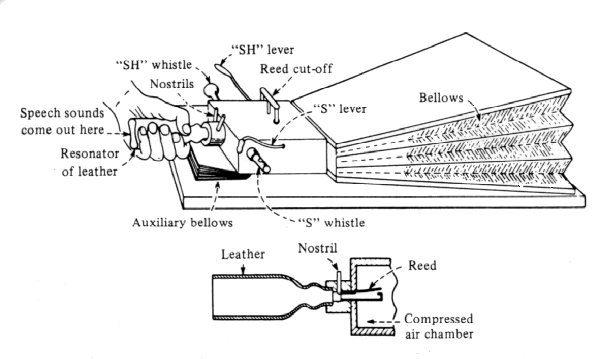
\includegraphics[width=\textwidth]{images/von_kempelen_machine.jpg}
		\caption{\cite{flanagan_book}}
	\end{center}
\end{figure}